\section{Verteilungssicht}

\subsection{Infrastruktur -- Ebene 1}

Das Gesamtsystem wird mit Docker Compose betrieben. Alle Container befinden
sich im gemeinsamen Docker-Netzwerk \texttt{app-net}.

Nur das Frontend veröffentlicht mit Port~\texttt{4321} einen Port auf dem
Docker-Host. Es leitet Backend-Anfragen intern über
\texttt{http://api-gateway:8080} an das API Gateway weiter.

Die Services, Datenbanken und der MQTT-Broker sind ausschließlich innerhalb
des Docker-Netzwerks erreichbar. Der Product Service wird mit drei Replikaten
ausgeführt, auf die ein interner Nginx-Loadbalancer die Anfragen verteilt.
    {
    \renewcommand{\arraystretch}{1.4}

    \begin{table}[H]
        \centering
        \begin{tabularx}{\linewidth}{
                >{\bfseries\raggedright\arraybackslash}p{0.25\linewidth}
                >{\raggedright\arraybackslash}p{0.14\linewidth}
                >{\raggedright\arraybackslash}p{0.18\linewidth}
                >{\raggedright\arraybackslash}X
        }
            \toprule
            \rowcolor{tableHeaderColor}
            Container & Host-Port & Interner Port & Anmerkung \\
            \midrule

            Frontend &
            4321 &
            4321 &
            Einziger von außen erreichbarer Container. \\

            \rowcolor{tableRowColor}
            API Gateway &
            -- &
            8080 &
            Zentraler Backend-Einstieg, nur intern erreichbar. \\

            Auth, User und Order Service &
            -- &
            8080 &
            Nur innerhalb von \texttt{app-net} erreichbar. \\

            \rowcolor{tableRowColor}
            Product Service &
            -- &
            8082 &
            Drei Replikate, nur intern erreichbar. \\

            Product-Service-Proxy &
            -- &
            80 &
            Interner Nginx-Loadbalancer. \\

            \rowcolor{tableRowColor}
            Email Service &
            -- &
            -- &
            Kommunikation ausschließlich über MQTT. \\

            MQTT-Broker &
            -- &
            1883, 9001 &
            Nur innerhalb von \texttt{app-net} erreichbar. \\

            \rowcolor{tableRowColor}
            PostgreSQL-Datenbanken &
            -- &
            5432 &
            Je zustandsbehaftetem Service eine Instanz. \\

            \bottomrule
        \end{tabularx}

        \caption{Container- und Portübersicht}
        \label{tab:container-ports}
    \end{table}
}
\begin{figure}[H]
  \centering
  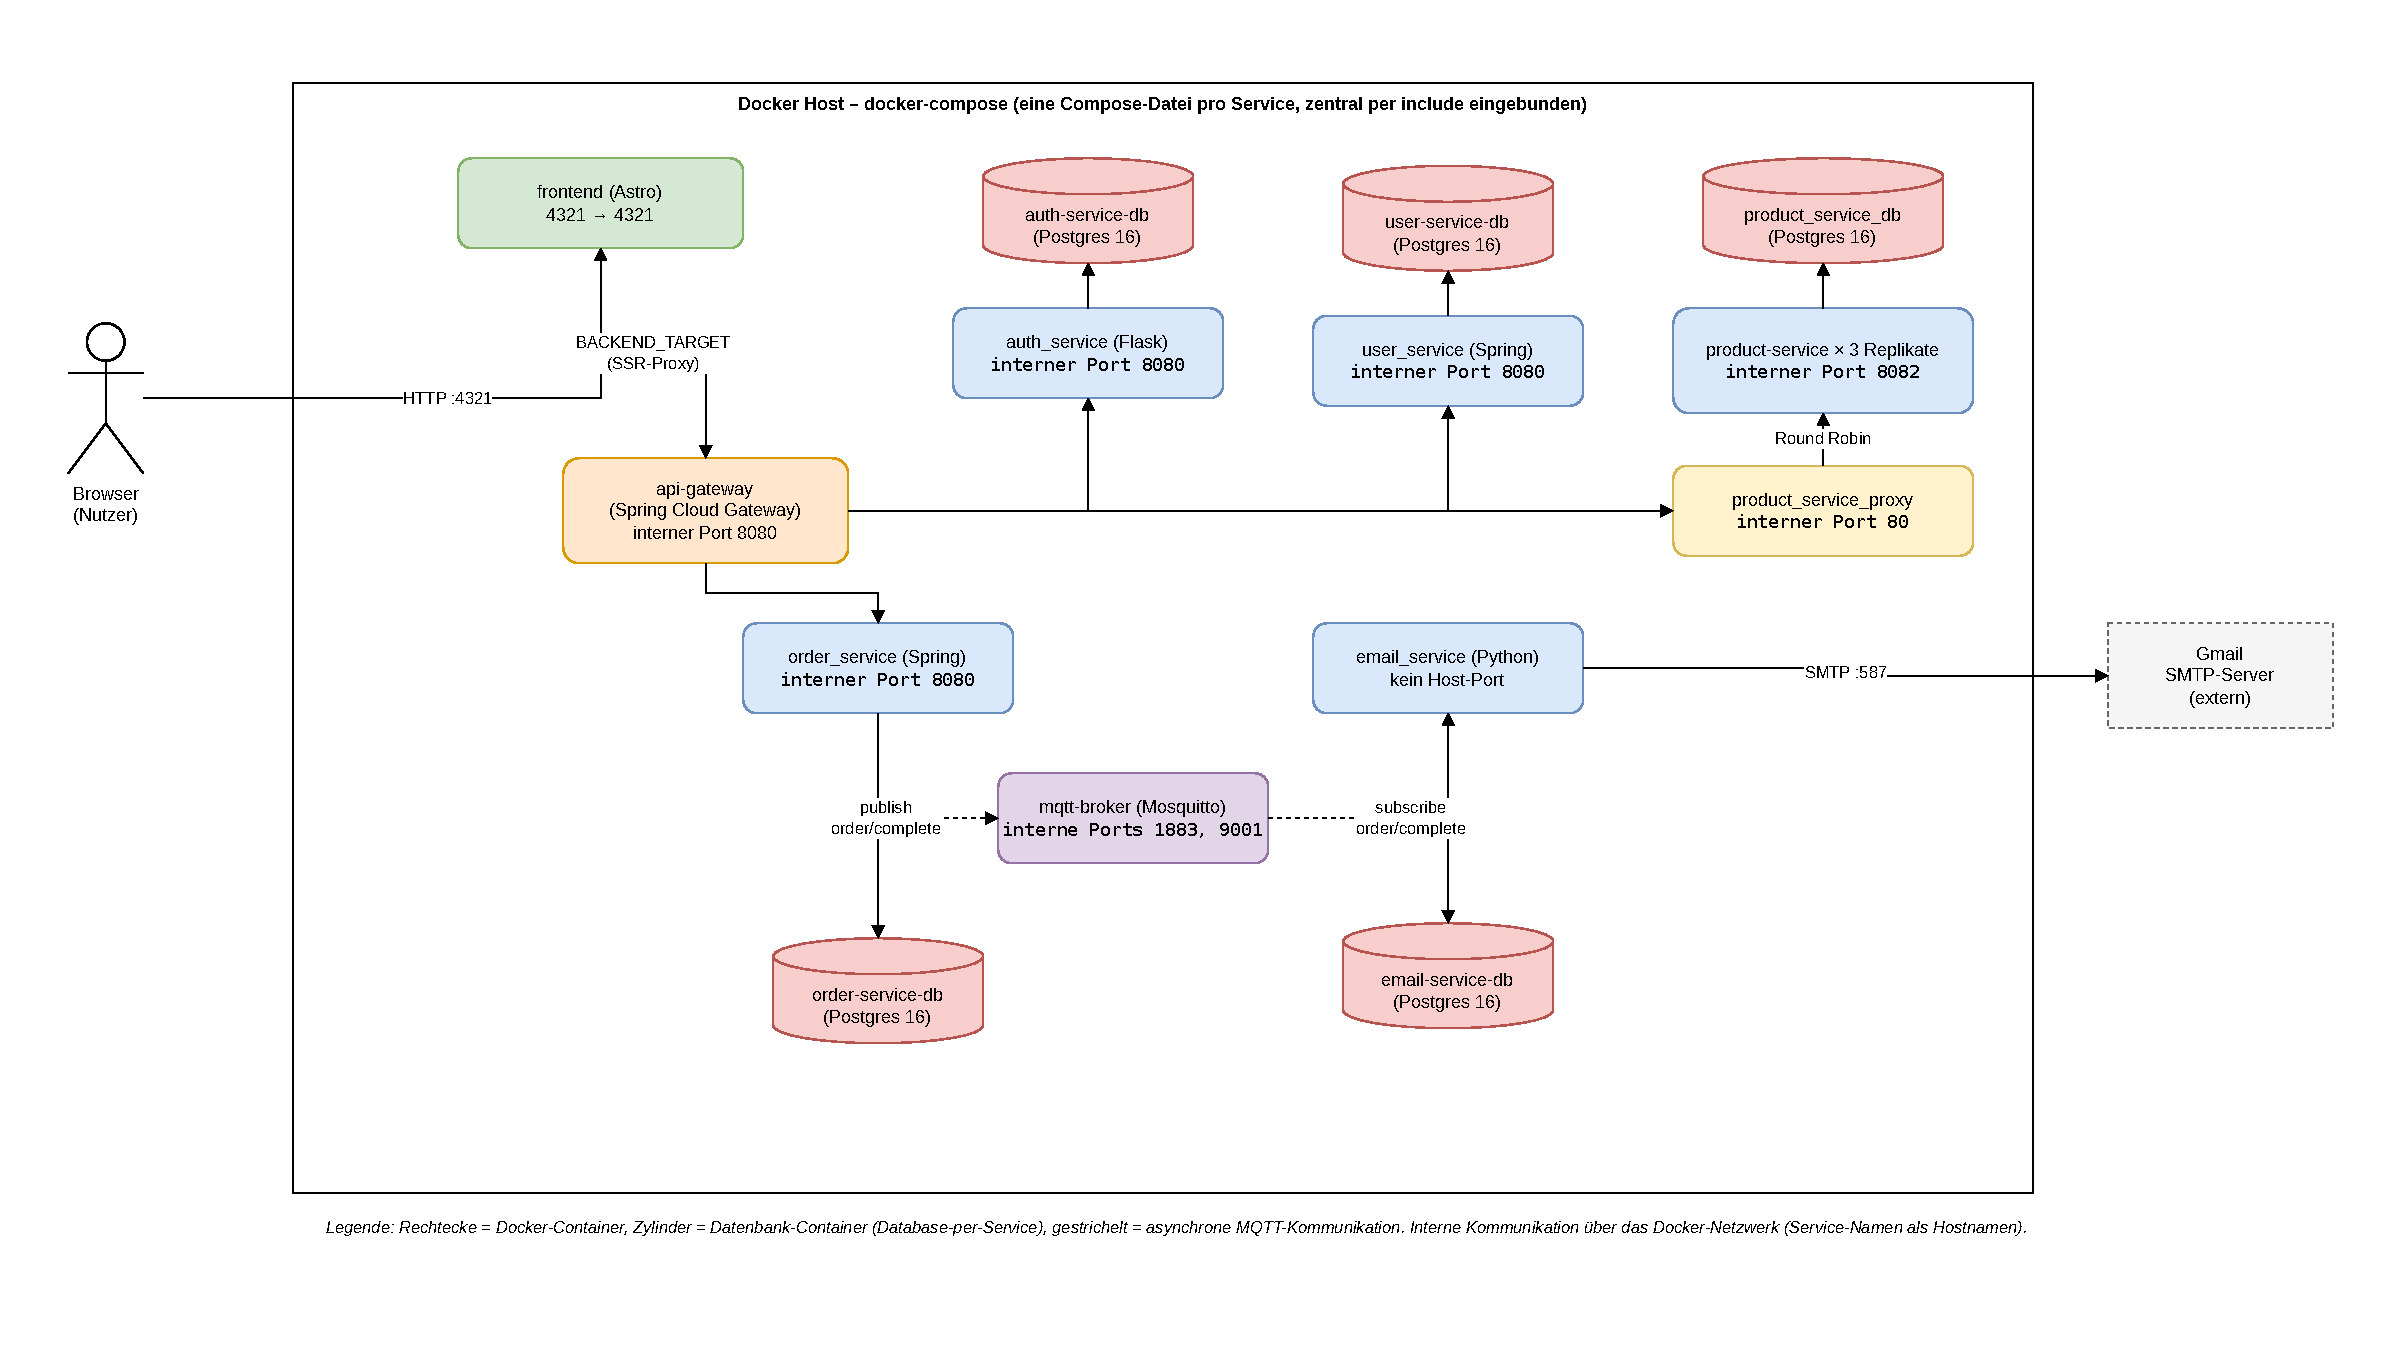
\includegraphics[width=\linewidth,trim=1cm 1.5cm 1cm 1cm,clip]{images/05-deployment}
  \caption{Deployment-Diagramm}
\end{figure}

